\section{System Description}
In this section, we describe our text processor and illustrate how we leverage pre-training word embedding and how to encode in our model. 
\begin{figure*}[t]
    \begin{center}
        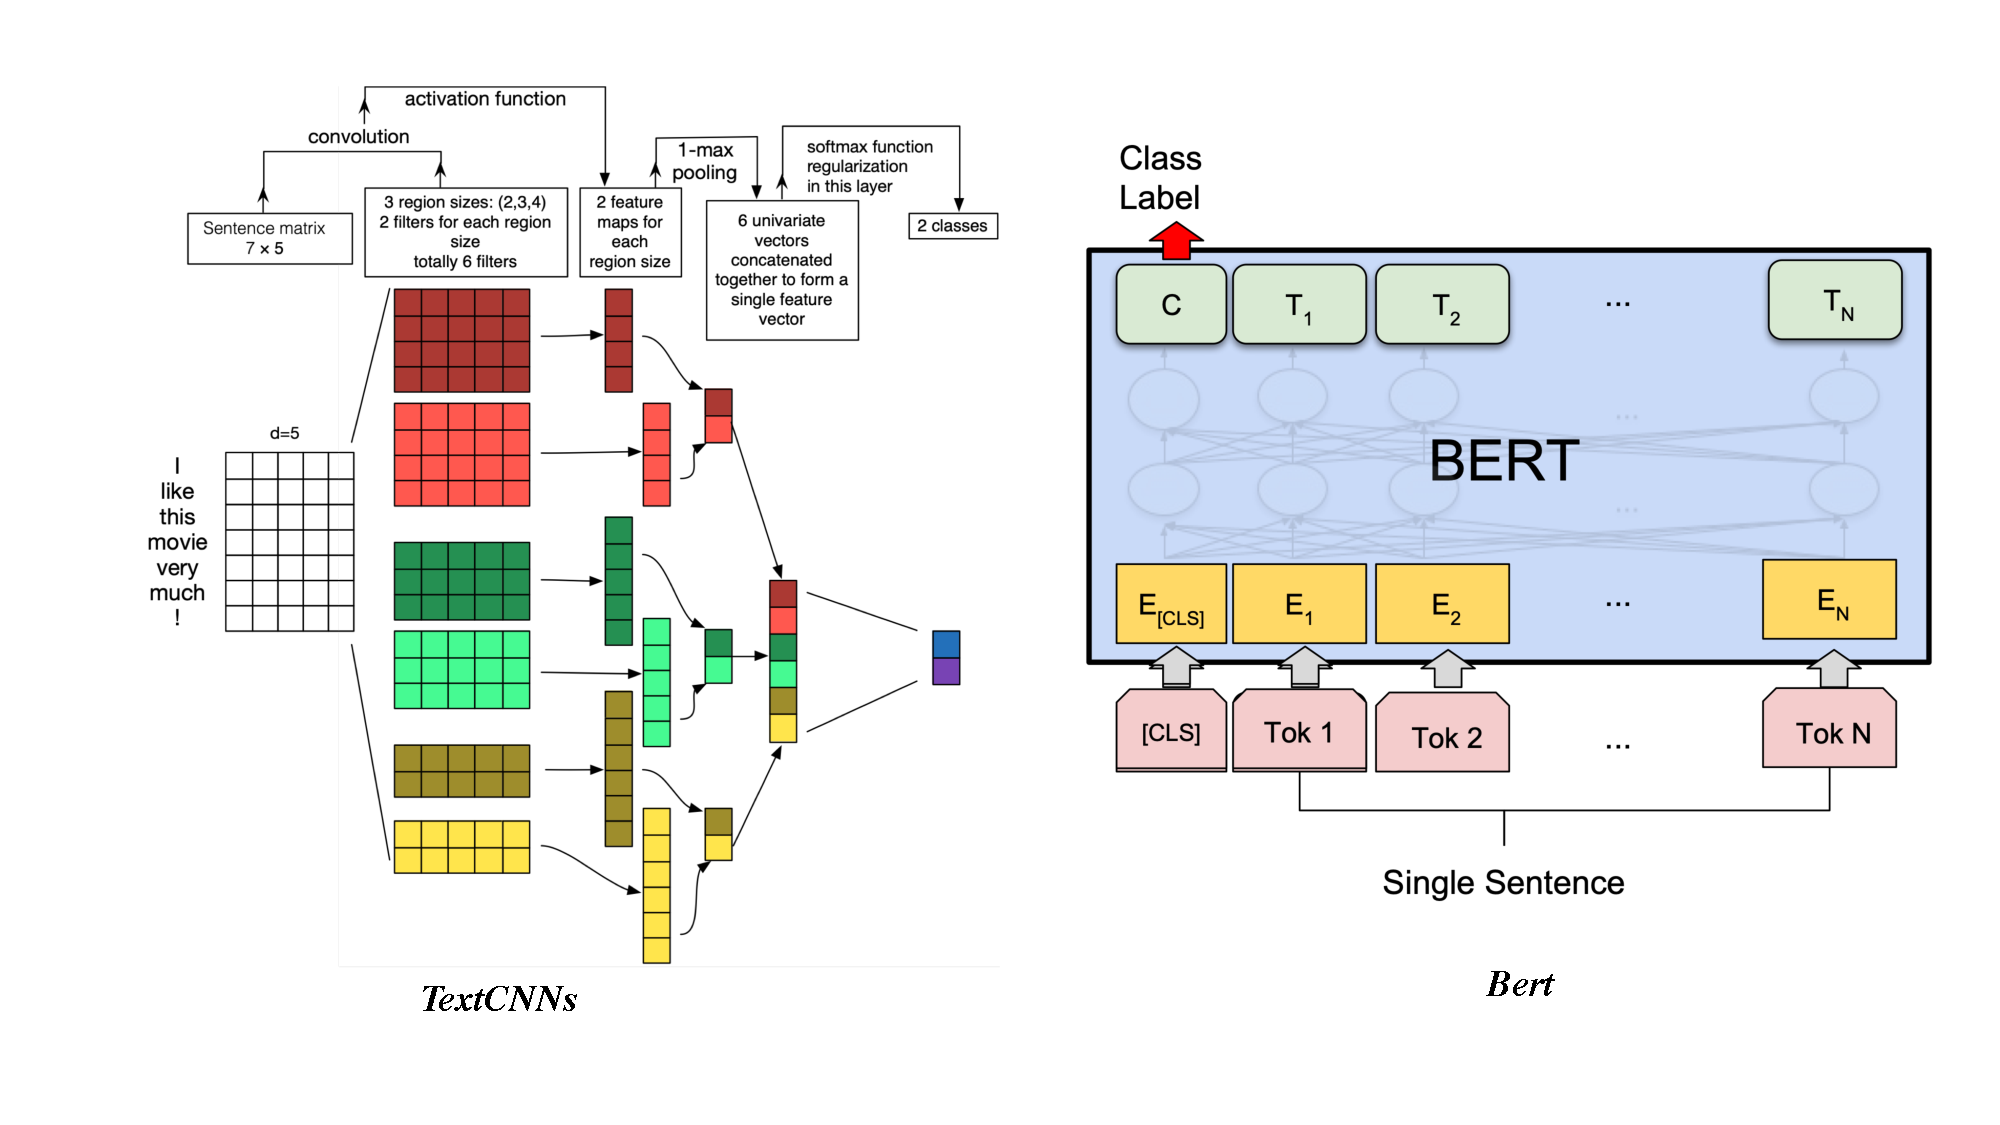
\includegraphics[width=\textwidth]{figures/figure.pdf}
    \end{center}
    \caption{Two model in this paper, TextCNN \& Bert}
    \label{fig:model}
\end{figure*}

    
\subsection{Text Processor}
The text processor reference by DataStroies \cite{biaziotis2017datastories}\footnote{github.com/cbaziotis/ekphrasis}. In this processor, we change emoji to a semantic word, change URL to label `$<$url$>$'. And we also lowercase all words and do some simple spell correction. This work can reduce the OOV situation. Before using the text processor, the ratio of OOV is 76.75\%(135619/177692). The ration of OOV using the text processor is 9.60\%(4491/45578). From this data, the text processing also reduces the word num.

After that, we alignment the sentences to max sentences line. In this processing, we add the pad to before first, after first, before the last one, after the lastest one respectively.

\subsection{Pre-training Embedding}

we pre-training the word embedding obtained from RepLab 2013 Dataset \cite{replab2013overview}\footnote{nlp.uned.es/replab2013/} about 9GB data. We train for word2vec \& fastText, having text processor, no text processor and respectively evaluation in LogisticRegression model. 


\subsection{TextCNN}

We first test in TextCNN model.  Its architecture is almost identical to CNN.  The input of the network are the tweets, which are tokenized into words which disposed of by text processor.  And each word is encoded by a word vector representation, i.e. a word embedding.  We also follow add zero-padding strategy such that all tweets have the same matrix dimension $X \in \mathbb{R}^{s'\times d}$, where we chose $s'=MaxSen.$=64(using TextProcessor)/35(no TextProcessor).  We then apply several convolution operations of various sizes to this matrix.  A single convolution involves a filtering matrix $w \in \mathbb{R}^{h\times d}$ where $h$ is the size of the convolution, meaning the number of words it spans.  The convolution operation is defined as 

\begin{eqnarray}
c_i &=& f \left( \sum_{j,k} w_{j,k} \left(X_{[i:i+h-1]} \right)_{j,k} + b \right)
\end{eqnarray}

where $b \in \mathbb{R}$ is a bias term and f(x) is a non-linear function, which we chose to be the `relu' function.  The output $c \in \mathbb{R}^{s'-h+1}$ is, therefore, a concatenation of the convolution operator over all possible window of words in the tweet. We can use multiple filtering matrices to learn different features, and additionally, we can use multiple convolution sizes to focus on smaller or larger regions of the tweets.  In practice, we used the filter size $[6,7,8]$ and we used a total of 256 filtering matrices for each filter size.\\

\subsection{Bert}

\begin{table*}[htbp!] % here top bottom page (! = remove further restrictions)
    \centering
    \begin{tabular}{llccccccc}
    \midrule
    Embedding Model  &  Text Processor          & Recall         & Precision       & Macro-F1        & Accuracy & Pos. &Neu. & Neg.\\
    \midrule
    no        & no           & 45.70   & 43.12     & 44.38    & 48.18    & 43.03 & \bf74.68    & 11.66 \\
    word2Vec  & no           & 44.87   & 42.48     & 43.65    & 51.37    & 60.81    & 57.27    & 9.37  \\
    fastText  & no           & 43.87   & 42.04     & 42.93    & 46.60    & 44.97    & 72.93    & 8.21  \\
    no        & ekphrasis    & 61.07   & 62.15     & 61.61    & 62.34 & \bf64.00    & 64.83    & 57.63 \\
    word2vec  & ekphrasis    & 61.49   & 62.35     & 61.92 & \bf64.37    & 62.52    & 68.72    & 55.80 \\
    fastText  & ekphrasis & \bf62.67 & 6\bf4.07 & \bf63.36    & 63.81    & 63.03    & 61.58 & \bf67.60 \\
    \bottomrule
    \end{tabular}
\caption{Comparison between different Embedding mode \& Text Processor using LibLinear logistic regression model on subtask A data (in \%)}
\label{tab:embedding}
\end{table*}

\begin{table*}[htbp!] % here top bottom page (! = remove further restrictions)
    \centering
    \begin{tabular}{rl}
    \midrule
        Sentences1:     &\textbf{\underline{Indian Mi Fans}}. Are Are Are \textbf{\underline{you}} ok? \\
        Sentences2:     &\textbf{\underline{Indian Mi Fans}}. Are \textbf{\underline{you}} ok? \\ 
        Before entity1: &\begin{scriptsize}[PAD] [PAD] \end{scriptsize} \textbf{\underline{Indian Mi Fans}}.  Are Are Are \textbf{\underline{you}} ok? \\
                        &\begin{scriptsize}[PAD] [PAD] [PAD] [PAD] \end{scriptsize}  \textbf{\underline{Indian Mi Fans}}. Are \textbf{\underline{you}} ok? \\
        After entity1:  &\textbf{\underline{Indian Mi Fans}}. \begin{scriptsize}[PAD] [PAD] \end{scriptsize} Are Are Are \textbf{\underline{you}} ok?\\
                        &\textbf{\underline{Indian Mi Fans}}. \begin{scriptsize}[PAD] [PAD] [PAD] [PAD] \end{scriptsize}  Are \textbf{\underline{you}} ok?\\
        Before entity2: &\textbf{\underline{Indian Mi Fans}}.  Are Are Are \begin{scriptsize}[PAD] [PAD] \end{scriptsize} \textbf{\underline{you}} ok? \\
                        &\textbf{\underline{Indian Mi Fans}}. Are \begin{scriptsize}[PAD] [PAD] [PAD] [PAD] \end{scriptsize}  \textbf{\underline{you}} ok? \\
        After entity2:  &\textbf{\underline{Indian Mi Fans}}. Are Are Are \textbf{\underline{you}} ok? \begin{scriptsize}[PAD] [PAD] \end{scriptsize} \\
                        &\textbf{\underline{Indian Mi Fans}}. Are \textbf{\underline{you}} ok? \begin{scriptsize}[PAD] [PAD] [PAD] [PAD] \end{scriptsize}  \\
    \bottomrule
    \end{tabular}
\caption{Pad example (MAX sentences size = 12)}
\label{tab:model}
\end{table*}

BERT is one of the key innovations in the recent progress of contextualized representation learning \cite{peters2018deep,howard2018universal,radford2018improving,devlin2018bert}.
The idea behind the progress is that even though the word embedding layer (in a typical neural network for NLP) is trained from large-scale corpora, training a wide variety of neural architectures that encode contextual representations only from the limited supervised data on end tasks is insufficient.
Unlike ELMo \cite{peters2018deep} and ULMFiT \cite{howard2018universal} that are intended to provide additional features for a particular architecture that bears human's understanding of the end task, BERT adopts a fine-tuning approach that requires almost no specific architecture for each end task. This is desired as an intelligent agent should minimize the use of prior human knowledge in the model design. Instead, it should learn such knowledge from data. BERT has two parameter intensive settings: 

\begin{itemize}
    \item {\bf \bertbase}: L=12, H=768, A=12, Total Parameters=110M
    \item {\bf \bertlarge}: L=24, H=1024, A=16, Total Parameters=340M
\end{itemize}